\subsection{Gini coefficient}

As mentioned in Section~\ref{giniKindaSucks}, the Gini coefficient is not the ideal measure of inequality for our apocalyptic model. Nonetheless, it is illustrative to see how it varies with respect to the ER $\lambda$ parameter. Figure~\ref{fig:giniVsLambda} depicts the Gini computed \textit{at the onset of stage 3} (before starvation) versus $\lambda$, and confirms that increasing $\lambda$ leads to a decreasing Gini coefficient. Increasing $\lambda$ fosters wealth uniformity through the increased formation of and growth in size of protos. Firstly, a higher percentage of agents join a proto as greater $\lambda$ values lead to fewer isolate agents in the ER network. As more agents join protos, differences in agent wealth are eliminated as each proto establishes perfect equality amongst its constituent agents, thereby lowering system's overall inequality. Secondly, higher $\lambda$ values lead to larger average proto sizes, as more densely-connected networks increase the likelihood that an agent will join an existing proto rather than form a new one. In much the same way, as smaller protos coalesce into larger ones, the standard inequality between the fragmented protos is eliminated in favor of perfect equality across the larger proto, resulting in a corresponding decrease in the Gini coefficient. 

\begin{figure}[hb]
\centering
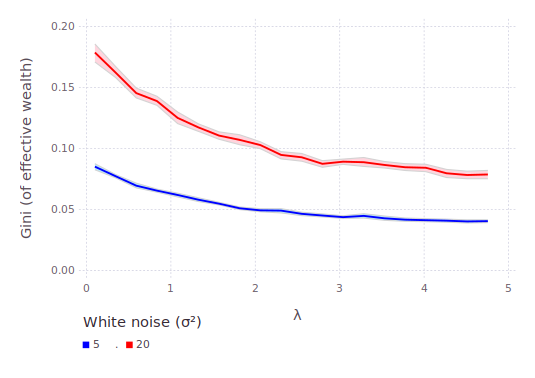
\includegraphics[width=\columnwidth]{figures/giniVsLambda.png}
\caption{The average Gini coefficient of effective wealth (computed pre-stage 3) for various values of the ER $\lambda$ connectivity parameter, and with both low-noise and high-noise income. 500 agents were used in each simulation. The color band represents a bootstrapped 95\% confidence interval.}
\label{fig:giniVsLambda}
\end{figure}

\subsection{Life expectancy}

Rather than absolute wealth, which the Gini coefficient measures, an alternate
measure of well-being is the ability to survive an economic downturn. This,
after all, is the chief benefit an agent should be able to expect from joining
a proto: it serves as a kind of insurance policy against future poverty. It is
therefore interesting to compare the life expectancy of agents who join protos
with those who do not.

There are many factors at play here, one of which is the level of white noise
($\sigma^2$) in the agents' income. Figure~\ref{fig:avgLifespanLambda} depicts
how the life expectancy of isolates and non-isolates depends on $\sigma^2$ for
two different values of $\lambda$. The top plot shows that for relatively
stable agent income levels, there is not much difference between the two lines
-- and hence, not much advantage (or disadvantage) to an agent's joining a
proto. Interestingly, however, the more volatile the income stream becomes, the
more benefit there is to pooling resources. The effect is even more pronounced
with more densely connected graphs, as in the bottom plot: here, when income is
more noisy, agents who join protos live nearly twice as long as those who
don't.

% Insert Rajesh's fascinating speculations about why this should be the case.


\begin{figure}[ht]
\centering
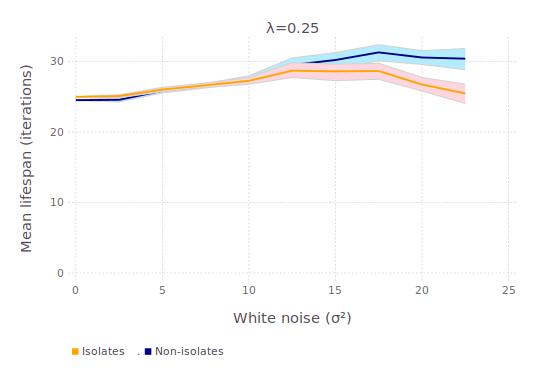
\includegraphics[width=\columnwidth]{figures/avgLifespanLambda_025.png}
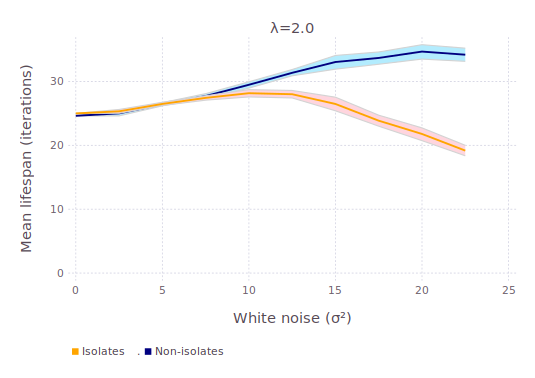
\includegraphics[width=\columnwidth]{figures/avgLifespanLambda2.png}
\caption{Life expectancy comparison between isolates (non-proto members) and
non-isolates (proto members) for different values of $\lambda$ and $\sigma^2$.
The \texttt{salary} parameter was set to 20, so the x-axis ranges from a nearly
constant agent income to a scenario when the noise is as high as the average.}
\label{fig:avgLifespanLambda}
\end{figure}

% Wealth histogram is steady ?
% vim:textwidth=99999
